% Hlavicka pro protokoly z fyzikalniho praktika.
% Verze pro: LaTeX
% Verze hlavicky: 22. 2. 2007
% Autor: Ustav fyziky kondenzovanych latek
% Ke stazeni: www.physics.muni.cz/ufkl/Vyuka/
% Licence: volne k pouziti, nejlepe k vcasnemu odevzdani protokolu z Vaseho mereni.

\documentclass[a4paper,11pt]{article}

% Kodovani (cestiny) v dokumentu: cp1250
% \usepackage[cp1250]{inputenc}	% Omezena stredoevropska kodova stranka, pouze MSW.
\usepackage[utf8]{inputenc}	% Doporucujeme pouzivat UTF-8 (unicode).
\usepackage{subfig}
\usepackage{float}

\usepackage{xparse}

\NewDocumentCommand{\codeword}{v}{%
\texttt{\textcolor{codepurple}{#1}}%
}

%%% Nemente:
\usepackage[margin=2cm]{geometry}
\newtoks\jmenopraktika \newtoks\jmeno \newtoks\datum
\newtoks\obor \newtoks\skupina \newtoks\rocnik \newtoks\semestr
\newtoks\cisloulohy \newtoks\jmenoulohy
\newtoks\tlak \newtoks\teplota \newtoks\vlhkost
%%% Nemente - konec.


%%%%%%%%%%% Doplnte pozadovane polozky:

\jmenopraktika={Fyzikální praktikum 1}  % nahradte jmenem vaseho predmetu
\jmeno={Milan Suk}            % nahradte jmenem mericiho
\datum={5. března 2018}        % nahradte datem mereni ulohy
\obor={F}                     % nahradte zkratkou vami studovaneho oboru
\skupina={PO 8:00}            % nahradte dobou vyuky vasi seminarni skupiny
\rocnik={I}                  % nahradte rocnikem, ve kterem studujete
\semestr={II}                 % nahradte semestrem, ve kterem studujete

\cisloulohy={2}               % nahradte cislem merene ulohy
\jmenoulohy={Meření odporu rezistoru} % nahradte jmenem merene ulohy

\tlak={97,9}                   % nahradte tlakem pri mereni (v hPa)
\teplota={21,4}               % nahradte teplotou pri mereni (ve stupnich Celsia)
\vlhkost={40}               % nahradte vlhkosti vzduchu pri mereni (v %)

%%%%%%%%%%% Konec pozadovanych polozek.


%%%%%%%%%%% Uzitecne balicky:
\usepackage[czech]{babel}
\usepackage{graphicx}
\usepackage{amsmath}
\usepackage{xspace}
\usepackage{url}
\usepackage{indentfirst}
\usepackage{listings}
\usepackage{color}


\definecolor{codegreen}{rgb}{0,0.6,0}
\definecolor{codegray}{rgb}{0.5,0.5,0.5}
\definecolor{codepurple}{rgb}{0.58,0,0.82}
\definecolor{backcolour}{rgb}{0.95,0.95,0.92}
 
\lstdefinestyle{mystyle}{
    backgroundcolor=\color{backcolour},   
    commentstyle=\color{codegreen},
    keywordstyle=\color{magenta},
    numberstyle=\tiny\color{codegray},
    stringstyle=\color{codepurple},
    basicstyle=\footnotesize,
    breakatwhitespace=false,         
    breaklines=true,                 
    captionpos=b,                    
    keepspaces=true,                 
    numbers=left,                    
    numbersep=5pt,                  
    showspaces=false,                
    showstringspaces=false,
    showtabs=false,                  
    tabsize=2
}
 
\lstset{style=mystyle}

%%%%%% Zamezeni parchantu:
\widowpenalty 10000 \clubpenalty 10000 \displaywidowpenalty 10000
%%%%%% Parametry pro moznost vsazeni vetsiho poctu obrazku na stranku
\setcounter{topnumber}{3}	  % max. pocet floatu nahore (specifikace t)
\setcounter{bottomnumber}{3}	  % max. pocet floatu dole (specifikace b)
\setcounter{totalnumber}{6}	  % max. pocet floatu na strance celkem
\renewcommand\topfraction{0.9}	  % max podil stranky pro floaty nahore
\renewcommand\bottomfraction{0.9} % max podil stranky pro floaty dole
\renewcommand\textfraction{0.1}	  % min podil stranky, ktery musi obsahovat text
\intextsep=8mm \textfloatsep=8mm  %\intextsep pro ulozeni [h] floatu a \textfloatsep pro [b] or [t]

% Tecky za cisly sekci:
\renewcommand{\thesection}{\arabic{section}.}
\renewcommand{\thesubsection}{\thesection\arabic{subsection}.}
% Jednopismenna mezera mezi cislem a nazvem kapitoly:
\makeatletter \def\@seccntformat#1{\csname the#1\endcsname\hspace{1ex}} \makeatother


%%%%%%%%%%%%%%%%%%%%%%%%%%%%%%%%%%%%%%%%%%%%%%%%%%%%%%%%%%%%%%%%%%%%%%%%%%%%%%%
%%%%%%%%%%%%%%%%%%%%%%%%%%%%%%%%%%%%%%%%%%%%%%%%%%%%%%%%%%%%%%%%%%%%%%%%%%%%%%%
% Zacatek dokumentu
%%%%%%%%%%%%%%%%%%%%%%%%%%%%%%%%%%%%%%%%%%%%%%%%%%%%%%%%%%%%%%%%%%%%%%%%%%%%%%%
%%%%%%%%%%%%%%%%%%%%%%%%%%%%%%%%%%%%%%%%%%%%%%%%%%%%%%%%%%%%%%%%%%%%%%%%%%%%%%%

\begin{document}

%%%%%%%%%%%%%%%%%%%%%%%%%%%%%%%%%%%%%%%%%%%%%%%%%%%%%%%%%%%%%%%%%%%%%%%%%%%%%%%
% Nemente:
%%%%%%%%%%%%%%%%%%%%%%%%%%%%%%%%%%%%%%%%%%%%%%%%%%%%%%%%%%%%%%%%%%%%%%%%%%%%%%%
\thispagestyle{empty}

{
\begin{center}
\sf 
{\Large Ústav fyzikální elektroniky Přírodovědecké fakulty Masarykovy univerzity} \\
\bigskip
{\huge \bfseries FYZIKÁLNÍ PRAKTIKUM} \\
\bigskip
{\Large \the\jmenopraktika}
\end{center}

\bigskip

\sf
\noindent
\setlength{\arrayrulewidth}{1pt}
\begin{tabular*}{\textwidth}{@{\extracolsep{\fill}} l l}
\large {\bfseries Zpracoval:}  \the\jmeno & \large  {\bfseries Naměřeno:} \the\datum\\[2mm]
\large  {\bfseries Obor:} \the\obor  \hspace{40mm}  {\bfseries Skupina:} \the\skupina %
&\large {\bfseries Testováno:}\\
\\
\hline
\end{tabular*}
}

\bigskip

{
\sf
\noindent \begin{tabular}{p{3cm} p{0.6\textwidth}}
\Large  Úloha č. {\bfseries \the\cisloulohy:} \par
&\Large \bfseries \the\jmenoulohy  \\[2mm]
\end{tabular}
}

%%%%%%%%%%%%%%%%%%%%%%%%%%%%%%%%%%%%%%%%%%%%%%%%%%%%%%%%%%%%%%%%%%%%%%%%%%%%%%%
% konec Nemente.
%%%%%%%%%%%%%%%%%%%%%%%%%%%%%%%%%%%%%%%%%%%%%%%%%%%%%%%%%%%%%%%%%%%%%%%%%%%%%%%

%%%%%%%%%%%%%%%%%%%%%%%%%%%%%%%%%%%%%%%%%%%%%%%%%%%%%%%%%%%%%%%%%%%%%%%%%%%%%%%
%%%%%%%%%%%%%%%%%%%%%%%%%%%%%%%%%%%%%%%%%%%%%%%%%%%%%%%%%%%%%%%%%%%%%%%%%%%%%%%
% Zacatek textu vlastniho protokolu
%%%%%%%%%%%%%%%%%%%%%%%%%%%%%%%%%%%%%%%%%%%%%%%%%%%%%%%%%%%%%%%%%%%%%%%%%%%%%%%
%%%%%%%%%%%%%%%%%%%%%%%%%%%%%%%%%%%%%%%%%%%%%%%%%%%%%%%%%%%%%%%%%%%%%%%%%%%%%%%


\section{Úvod}

    \paragraph{} Cílem tohoto měření bylo zjistit odpor určených rezistorů. V 
    metodě A voltmetr přímo měří napětí na rezistoru, ale ampérmetr měří proud,
    který se dělí do větví $I_{V}$ a $I_{R}$. Výsledný odpor se určí následující
    rovnice

    \begin{equation}
        R = \frac{U_{V}}{I_{A} - \frac{U_{V}}{R_{V}}}
    \end{equation}

    \begin{figure}[H]
        \centering
        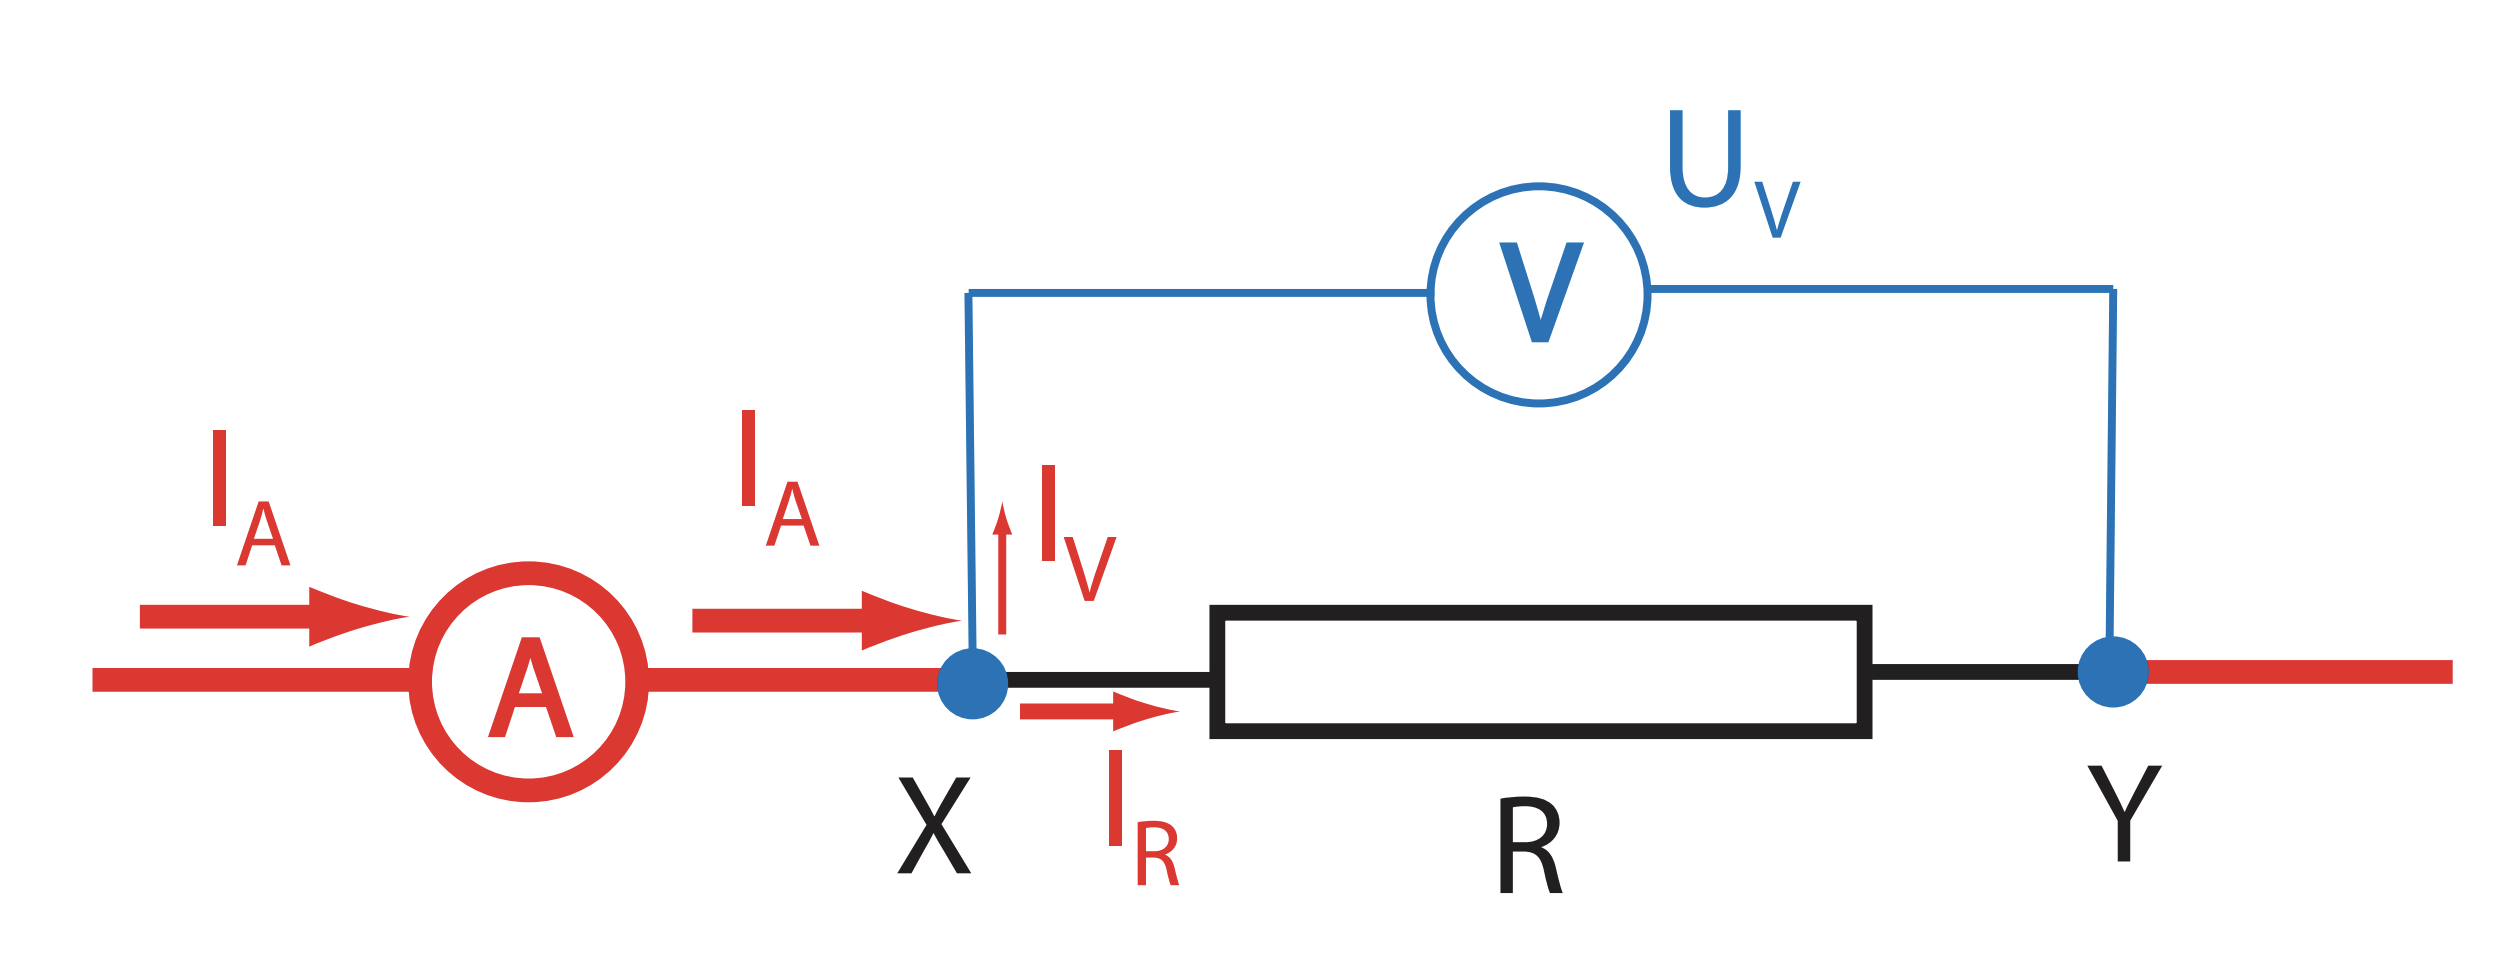
\includegraphics[width=0.6\linewidth]{metoda_A.png}
        \caption{Metoda A}
    \end{figure}

    \paragraph{} Při druhé metodě ampérmetr měří správný proud, ale volmetr 
    měří napětí na rezistoru a ampérmetr zároveň. V tomto případě se odpor 
    určí jako

    \begin{equation}
        R = \frac{U_{V}}{I_{A}} - R_{A}
    \end{equation}

    \begin{figure}[H]
        \centering
        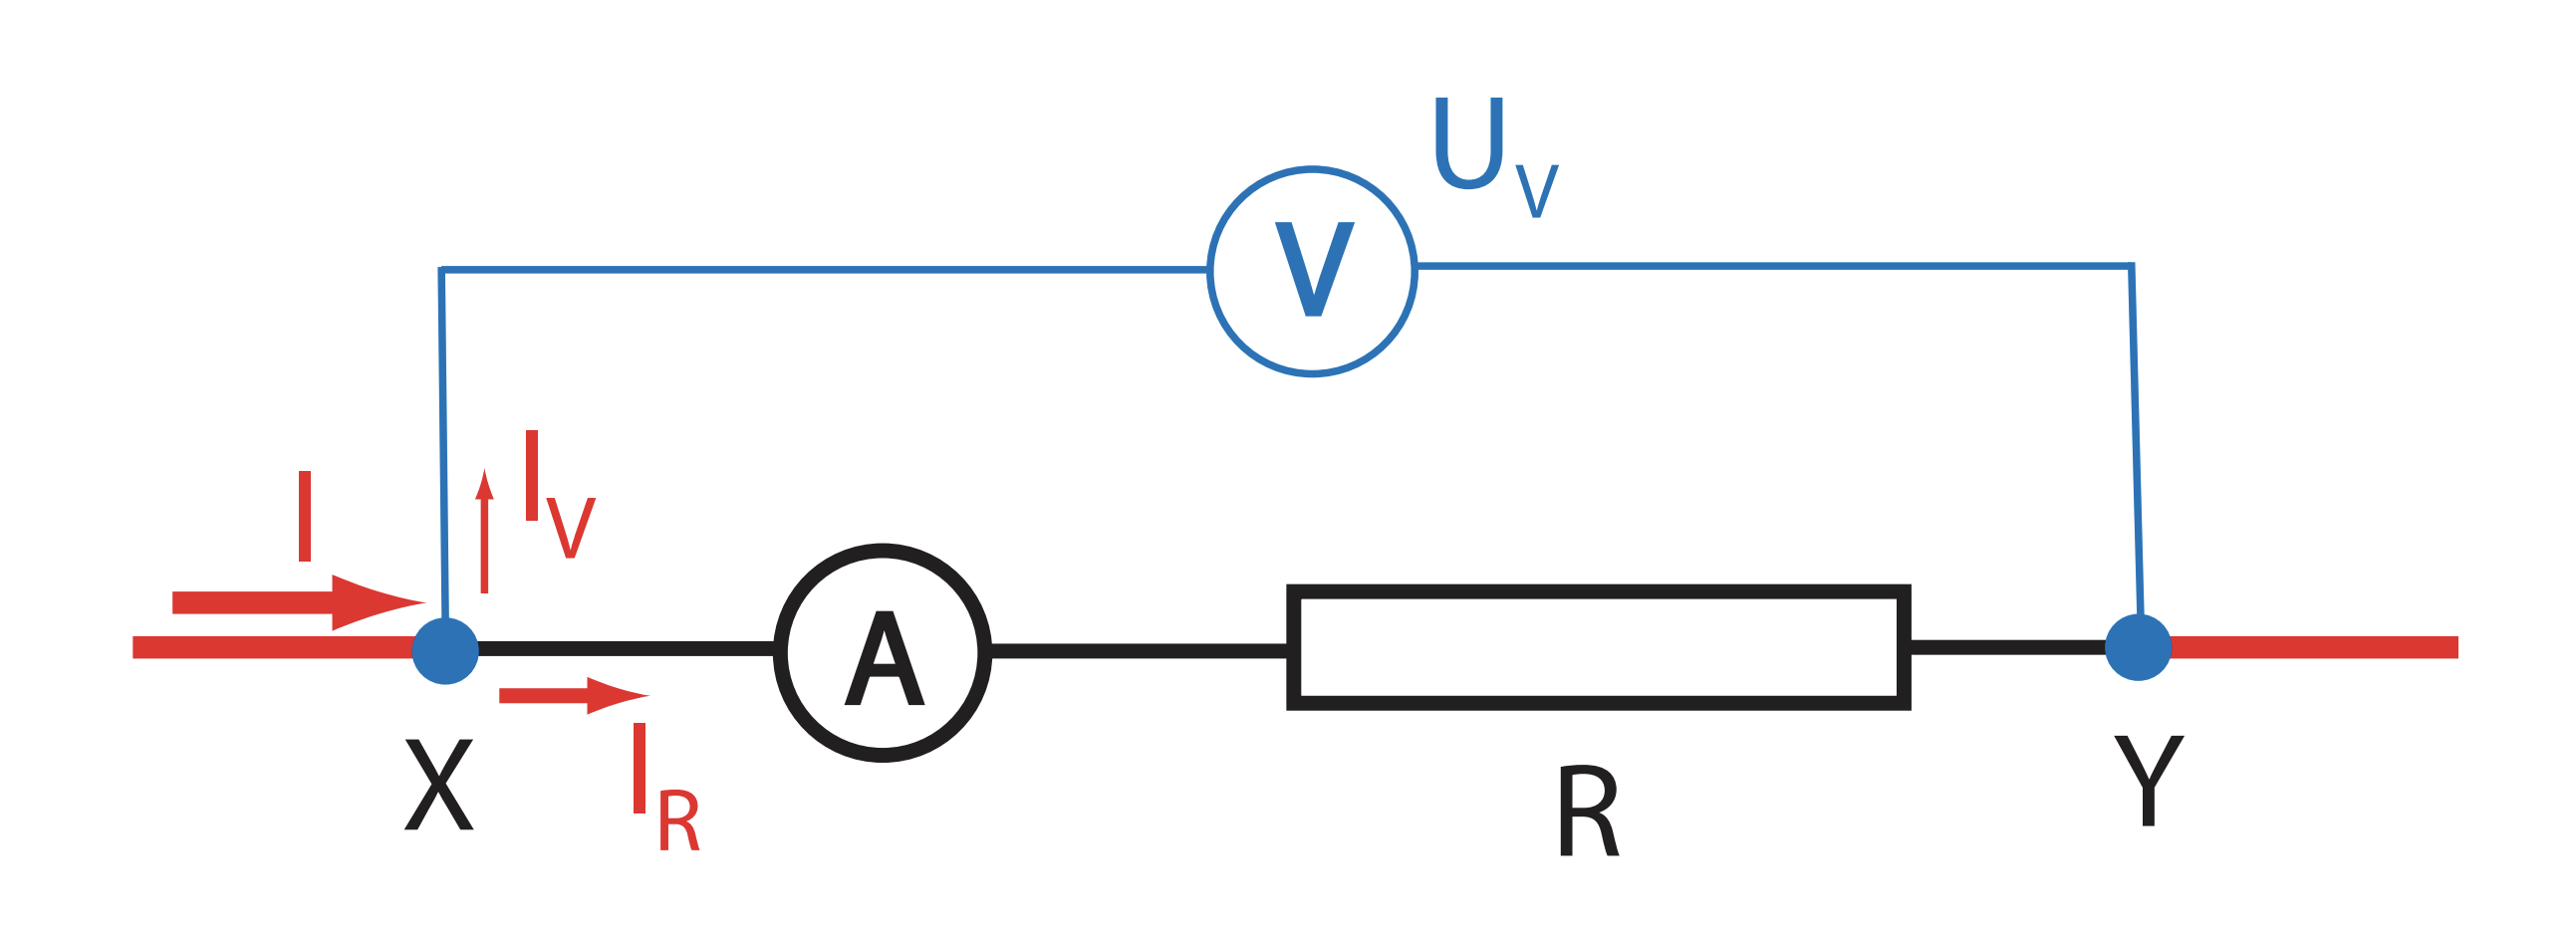
\includegraphics[width=0.6\linewidth]{metoda_B.png}
        \caption{Metoda B}
    \end{figure}

\section{Měření}

    \paragraph{} Pro zpracování výsledků použiji následující skript, který
    generuje grafy závislosti napětí na proudu a zároveň poučítá regresy, z
    které můžu určit hodnotu odporu.

\begin{lstlisting}[language=Python][h]
import matplotlib.pyplot as plt
from scipy import stats
import numpy

def add(filename, curve_type):
    data = numpy.loadtxt(filename, delimiter=';')

    data_x = [x[0] * 0.001 for x in data]
    data_y = [x[1] for x in data]

    slope, intercept, r_value, p_value, std_err = stats.linregress(
        data_x, data_y)

    regression_x = data_x
    regression_y = [slope * x + intercept for x in regression_x]

    plt.plot(data_x, data_y, curve_type)
    plt.plot(regression_x, regression_y, '-')

if __name__ == '__main__':
    add("A__1", 'ro') # zde staci nahradit za soubor B__1
    add("A__2", 'bo') # zde staci nahradit za soubor B__2

    plt.ylabel('Napeti [V]')
    plt.xlabel('Proud [A]')
    plt.show()\end{lstlisting} 

    \begin{figure}[H]
        \centering
        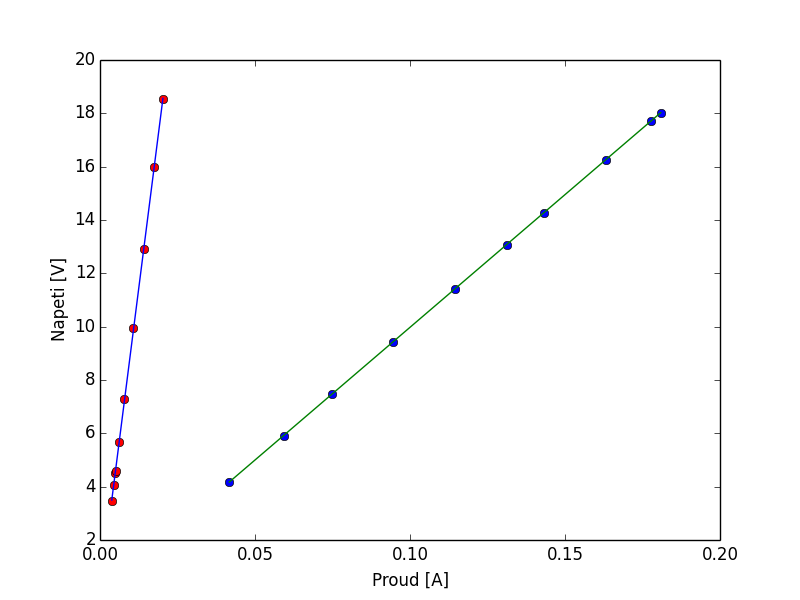
\includegraphics[width=0.6\linewidth]{A.png}
        \caption{Metoda A}
    \end{figure}

\begin{lstlisting}[language=Bash][H]
A__1: R = 904.55143625 +- 1.78768667796
A__2: R = 99.4162472948 +- 0.0276436922162\end{lstlisting}

    \paragraph{} Pro metodu A vycházejí odpory

    \begin{equation}
        R^{(A)}_{1} = (904 \pm 2) \Omega
    \end{equation}
    \begin{equation}
        R^{(A)}_{2} = (99.42 \pm 0.03) \Omega
    \end{equation}

    \begin{figure}[H]
        \centering
        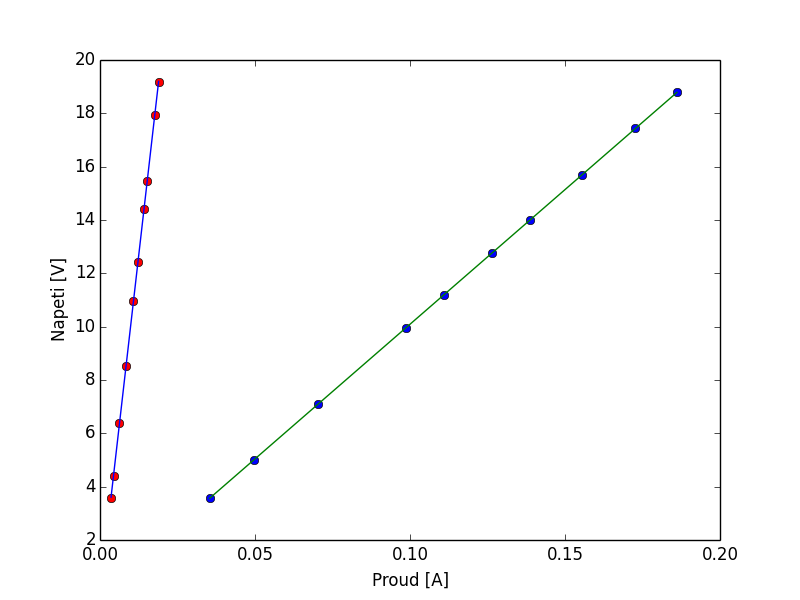
\includegraphics[width=0.6\linewidth]{B.png}
        \caption{Metoda B}
    \end{figure}

\begin{lstlisting}[language=Bash][H]
A__1: R = 912.807993713 +- 1.82047192985
A__2: R = 99.5151814925 +- 0.0276987389312\end{lstlisting}

    \paragraph{} Pro metodu B vycházejí odpory

    \begin{equation}
        R^{(B)}_{1} = (913 \pm 2) \Omega
    \end{equation}
    \begin{equation}
        R^{(B)}_{2} = (99.51 \pm 0.03) \Omega
    \end{equation}

    \paragraph{} Pro žárovku jsem postupoval obdobně.

    \begin{figure}[H]
        \centering
        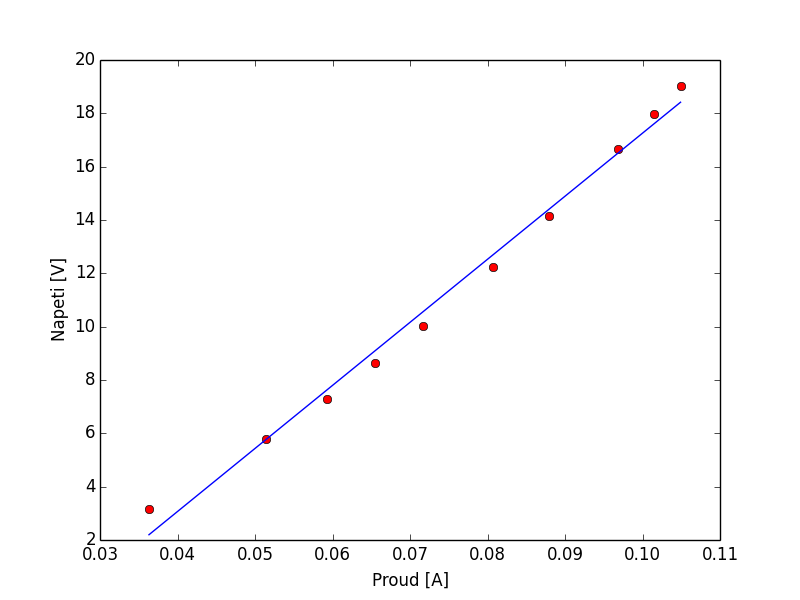
\includegraphics[width=0.6\linewidth]{C.png}
        \caption{Měření voltampérové charakteristiky žárovky}
    \end{figure}

\begin{lstlisting}[language=Bash][H]
A__3: R = 236.463736856 +- 7.9588549935\end{lstlisting}

    \begin{equation}
        R^{(Z)} = (236 \pm 8) \Omega
    \end{equation}

    \paragraph{} Při mětodě A jsem řešil dělení proudu do větvý 
    modifikací dat při výpočtu regrese. Každý záznam proudu jsem
    následujícím kódem v každém bodě zvětšil o odebraný proud
    do větve s voltmetrem.
    

\begin{lstlisting}[language=Bash][H]
for i in range(len(data_x)):
    data_x[i] = data_x[i] + data_y[i] / R_V\end{lstlisting}

    \paragraph{} Naopak u metody B postačilo k výslednému proudu
    přičíst vnitřní odpor ampérmetr.

\end{document}
